\documentclass[journal]{IEEEtran} 
\usepackage[T1]{fontenc}
\usepackage{lmodern}
\usepackage[utf8]{inputenc}
\usepackage{graphicx}
\usepackage{amsmath,amssymb}
\usepackage{booktabs}
\usepackage{siunitx}
\usepackage{hyperref}
\usepackage{cite}

\usepackage{tikz}
\usetikzlibrary{arrows.meta,positioning,fit}

\graphicspath{{./}}

\title{A Comparative Review of DRAM and FeRAM: The Boundary between Volatile and Non-Volatile Memory and Future Perspectives}

\author{Shinichi~Samizo%
\thanks{S. Samizo is with Project Design Hub (Samizo-AITL), Japan. E-mail: \texttt{samizo-aitl@example.org}.}
}

\markboth{Draft for IEEE-style submission}{Samizo: DRAM vs FeRAM Comparative Review}

\begin{document}
\maketitle

\begin{abstract}
Dynamic Random-Access Memory (DRAM) has served as the workhorse of volatile memory technology for decades, while Ferroelectric Random-Access Memory (FeRAM), particularly HfO$_2$-based devices, has emerged as a promising non-volatile alternative. This review provides a comparative analysis of DRAM and FeRAM in terms of scaling trends, device reliability, and system-level implications. Key metrics such as access speed, retention time, endurance, and energy per bit are summarized in Table~\ref{tab:comparison}, while Figs.~\ref{fig:dram_evolution}--\ref{fig:hybrid_hierarchy} illustrate the trade-offs and perspectives. Finally, we highlight hybrid scenarios where DRAM and FeRAM may co-exist in future memory hierarchies, and discuss challenges for bridging the volatile--non-volatile boundary.
\end{abstract}

\begin{IEEEkeywords}
DRAM, FeRAM, FeFET, HfO$_2$, reliability, retention, endurance, scaling, memory hierarchy, review.
\end{IEEEkeywords}

\section{Introduction}

\noindent
Memory hierarchies are critical to modern computing systems. DRAM remains the dominant volatile memory owing to its high speed and scalability, whereas FeRAM (including FeFET-based cells) offers non-volatility with competitive speed. This review targets researchers and practitioners by consolidating recent results from IEDM/VLSI and IEEE journals, and by proposing a hybrid perspective that redefines the boundary between volatile and non-volatile memory.

% test build



\section{DRAM Technology and Scaling}
DRAM technology has continually advanced through cell capacitor scaling, high-k dielectrics, and process innovations. 
Recent works highlight the difficulty of maintaining capacitance while suppressing leakage currents in deep sub-20 nm technologies \cite{choi2022}.
Furthermore, the industry is exploring 3D DRAM architectures to extend scaling, analogous to NAND flash, by stacking capacitor arrays \cite{kim2021_dram}.
Such approaches aim to overcome cell aspect ratio limits, though integration complexity and refresh overhead remain unresolved.

\begin{figure}[!t]
\centering
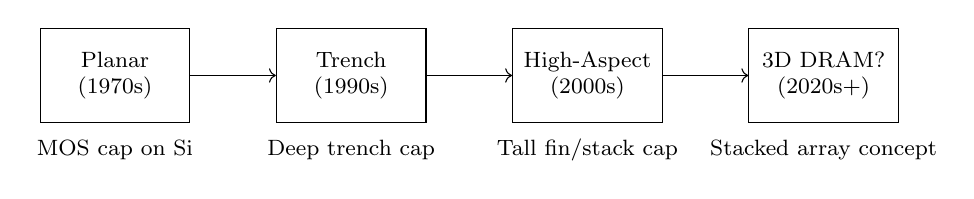
\begin{tikzpicture}[font=\footnotesize]
% ノード(座標配置・すべて align=center)
\node[draw, minimum width=1.9cm, minimum height=1.2cm, align=center] (planar) at (0,0) {Planar\\(1970s)};
\node[draw, minimum width=1.9cm, minimum height=1.2cm, align=center] (trench) at (3,0) {Trench\\(1990s)};
\node[draw, minimum width=1.9cm, minimum height=1.2cm, align=center] (hac)    at (6,0) {High-Aspect\\(2000s)};
\node[draw, minimum width=1.9cm, minimum height=1.2cm, align=center] (ddram)  at (9,0) {3D DRAM?\\(2020s+)};

% 矢印
\draw[->] (planar) -- (trench);
\draw[->] (trench) -- (hac);
\draw[->] (hac) -- (ddram);

% 注記
\node[align=center] at (0,-0.95) {MOS cap on Si};
\node[align=center] at (3,-0.95) {Deep trench cap};
\node[align=center] at (6,-0.95) {Tall fin/stack cap};
\node[align=center] at (9,-0.95) {Stacked array concept};
\end{tikzpicture}
\caption{Evolution of DRAM cell structures and concepts.}
\label{fig:dram_evolution}
\end{figure}


\section{FeRAM Technology and Advances}
The discovery of ferroelectricity in HfO$_2$ thin films~\cite{boscke2011} revitalized FeRAM research, enabling aggressive scaling and compatibility with CMOS back-end processes. 
FeFET devices integrate ferroelectric layers directly into the gate stack, offering non-volatile operation with near-DRAM speed~\cite{mueller2012}. 
Nevertheless, challenges persist in retention, fatigue, and variability, especially under scaled dimensions~\cite{schenk2015, kim2020_fefet}. 
Recent progress has improved endurance beyond $10^{12}$ cycles and enhanced retention stability in scaled FeFETs~\cite{li2022}. 
Reliability studies further emphasize the role of defect generation and TDDB under high-field operation~\cite{park2019_tddb}.
Despite progress, device variability~\cite{kim2020_fefet} and TDDB-related degradation~\cite{park2019_tddb} 
remain major reliability bottlenecks. 
Endurance improvements beyond $10^{12}$ cycles~\cite{li2022} suggest promising scaling paths, 
though retention degradation under aggressive field stress continues to be investigated~\cite{schenk2015}.


\section{Comparative Analysis: DRAM vs FeRAM}
\label{sec:comparison}
Table~\ref{tab:comparison} summarizes representative metrics (speed, retention, endurance, energy/bit, and cell footprint) for DRAM and FeRAM. 

DRAM provides ultra-high endurance ($\geq 10^{16}$ cycles) and low energy/bit, but suffers from limited retention ($\sim$64 ms) and high refresh overhead. FeRAM, by contrast, offers non-volatility with retention exceeding $10^5$ s and endurance of $10^{12}$--$10^{13}$ cycles, but its write energy is higher (hundreds of fJ/bit) \cite{noheda2023,martin2020}. 

Fig.~\ref{fig:svr} shows the speed–retention map, while Fig.~\ref{fig:evs} highlights the trade-off between write energy and speed. These comparative plots illustrate that DRAM is optimal for working memory, whereas FeRAM is suitable for low-power non-volatile applications.


\section{Hybrid Perspectives and Future Memory Hierarchies}
\subsection*{Benefits}
\begin{itemize}
  \item \textbf{Reduced refresh overhead:} Part of the dataset can be parked in FeRAM, cutting DRAM refresh traffic and standby power.
  \item \textbf{Fast persistence:} System state can be checkpointed to FeRAM with microsecond-scale latency, enabling quick resume.
  \item \textbf{Data resilience:} FeRAM provides crash consistency for critical metadata and write-back buffers.
\end{itemize}

\subsection*{Constraints and trade-offs}
\begin{itemize}
  \item \textbf{Endurance and variability:} FeRAM endurance ($10^{12}$--$10^{13}$ cycles) is high but still below DRAM refresh activity.
  \item \textbf{Write energy and latency:} FeRAM generally incurs higher write energy than DRAM; policies should bias read-mostly or cold data to FeRAM.
  \item \textbf{Integration cost:} Adding FeFET or ferroelectric layers in advanced CMOS nodes introduces process-compatibility and reliability risks (e.g., TDDB under high fields).
\end{itemize}

\subsection*{System design directions}
\begin{itemize}
  \item \textbf{Tiering policies:} Classify pages/objects by write intensity and retention needs, migrating cold or persistent data to FeRAM.
  \item \textbf{Refresh co-optimization:} Dynamically shrink DRAM refresh for regions shadowed or backed by FeRAM.
  \item \textbf{Checkpoint and logging:} Exploit FeRAM bandwidth for low-latency state persistence.
  \item \textbf{Controller support:} Keep metadata for wear leveling, retention-aware placement, and error monitoring (e.g., soft/hard failure counters).
\end{itemize}


\section{Conclusion and Outlook}
Comparative analysis suggests that DRAM will continue as the workhorse volatile memory, maintaining unmatched endurance and density. 
Meanwhile, FeRAM offers a compelling pathway toward embedded non-volatile solutions with competitive speed and CMOS process compatibility~\cite{noheda2023, martin2020}. 
The convergence of DRAM and FeRAM within hybrid hierarchies could redefine system memory, but scaling, reliability, and integration challenges remain open research frontiers. 
Future work should focus on bridging device-level improvements with architecture-level deployment, ensuring that emerging ferroelectric memories can complement or eventually rival DRAM in mainstream applications.


% --- References ---
\nocite{*}
\bibliographystyle{IEEEtran}
\bibliography{references}

\end{document}

% rebuild
